
\documentclass{article} % For LaTeX2e
\usepackage{iclr_template/iclr2025_conference,times}

% Optional math commands from https://github.com/goodfeli/dlbook_notation.
%%%%% NEW MATH DEFINITIONS %%%%%

\usepackage{amsmath,amsfonts,bm}

% Mark sections of captions for referring to divisions of figures
\newcommand{\figleft}{{\em (Left)}}
\newcommand{\figcenter}{{\em (Center)}}
\newcommand{\figright}{{\em (Right)}}
\newcommand{\figtop}{{\em (Top)}}
\newcommand{\figbottom}{{\em (Bottom)}}
\newcommand{\captiona}{{\em (a)}}
\newcommand{\captionb}{{\em (b)}}
\newcommand{\captionc}{{\em (c)}}
\newcommand{\captiond}{{\em (d)}}

% Highlight a newly defined term
\newcommand{\newterm}[1]{{\bf #1}}


% Figure reference, lower-case.
\def\figref#1{figure~\ref{#1}}
% Figure reference, capital. For start of sentence
\def\Figref#1{Figure~\ref{#1}}
\def\twofigref#1#2{figures \ref{#1} and \ref{#2}}
\def\quadfigref#1#2#3#4{figures \ref{#1}, \ref{#2}, \ref{#3} and \ref{#4}}
% Section reference, lower-case.
\def\secref#1{section~\ref{#1}}
% Section reference, capital.
\def\Secref#1{Section~\ref{#1}}
% Reference to two sections.
\def\twosecrefs#1#2{sections \ref{#1} and \ref{#2}}
% Reference to three sections.
\def\secrefs#1#2#3{sections \ref{#1}, \ref{#2} and \ref{#3}}
% Reference to an equation, lower-case.
\def\eqref#1{equation~\ref{#1}}
% Reference to an equation, upper case
\def\Eqref#1{Equation~\ref{#1}}
% A raw reference to an equation---avoid using if possible
\def\plaineqref#1{\ref{#1}}
% Reference to a chapter, lower-case.
\def\chapref#1{chapter~\ref{#1}}
% Reference to an equation, upper case.
\def\Chapref#1{Chapter~\ref{#1}}
% Reference to a range of chapters
\def\rangechapref#1#2{chapters\ref{#1}--\ref{#2}}
% Reference to an algorithm, lower-case.
\def\algref#1{algorithm~\ref{#1}}
% Reference to an algorithm, upper case.
\def\Algref#1{Algorithm~\ref{#1}}
\def\twoalgref#1#2{algorithms \ref{#1} and \ref{#2}}
\def\Twoalgref#1#2{Algorithms \ref{#1} and \ref{#2}}
% Reference to a part, lower case
\def\partref#1{part~\ref{#1}}
% Reference to a part, upper case
\def\Partref#1{Part~\ref{#1}}
\def\twopartref#1#2{parts \ref{#1} and \ref{#2}}

\def\ceil#1{\lceil #1 \rceil}
\def\floor#1{\lfloor #1 \rfloor}
\def\1{\bm{1}}
\newcommand{\train}{\mathcal{D}}
\newcommand{\valid}{\mathcal{D_{\mathrm{valid}}}}
\newcommand{\test}{\mathcal{D_{\mathrm{test}}}}

\def\eps{{\epsilon}}


% Random variables
\def\reta{{\textnormal{$\eta$}}}
\def\ra{{\textnormal{a}}}
\def\rb{{\textnormal{b}}}
\def\rc{{\textnormal{c}}}
\def\rd{{\textnormal{d}}}
\def\re{{\textnormal{e}}}
\def\rf{{\textnormal{f}}}
\def\rg{{\textnormal{g}}}
\def\rh{{\textnormal{h}}}
\def\ri{{\textnormal{i}}}
\def\rj{{\textnormal{j}}}
\def\rk{{\textnormal{k}}}
\def\rl{{\textnormal{l}}}
% rm is already a command, just don't name any random variables m
\def\rn{{\textnormal{n}}}
\def\ro{{\textnormal{o}}}
\def\rp{{\textnormal{p}}}
\def\rq{{\textnormal{q}}}
\def\rr{{\textnormal{r}}}
\def\rs{{\textnormal{s}}}
\def\rt{{\textnormal{t}}}
\def\ru{{\textnormal{u}}}
\def\rv{{\textnormal{v}}}
\def\rw{{\textnormal{w}}}
\def\rx{{\textnormal{x}}}
\def\ry{{\textnormal{y}}}
\def\rz{{\textnormal{z}}}

% Random vectors
\def\rvepsilon{{\mathbf{\epsilon}}}
\def\rvtheta{{\mathbf{\theta}}}
\def\rva{{\mathbf{a}}}
\def\rvb{{\mathbf{b}}}
\def\rvc{{\mathbf{c}}}
\def\rvd{{\mathbf{d}}}
\def\rve{{\mathbf{e}}}
\def\rvf{{\mathbf{f}}}
\def\rvg{{\mathbf{g}}}
\def\rvh{{\mathbf{h}}}
\def\rvu{{\mathbf{i}}}
\def\rvj{{\mathbf{j}}}
\def\rvk{{\mathbf{k}}}
\def\rvl{{\mathbf{l}}}
\def\rvm{{\mathbf{m}}}
\def\rvn{{\mathbf{n}}}
\def\rvo{{\mathbf{o}}}
\def\rvp{{\mathbf{p}}}
\def\rvq{{\mathbf{q}}}
\def\rvr{{\mathbf{r}}}
\def\rvs{{\mathbf{s}}}
\def\rvt{{\mathbf{t}}}
\def\rvu{{\mathbf{u}}}
\def\rvv{{\mathbf{v}}}
\def\rvw{{\mathbf{w}}}
\def\rvx{{\mathbf{x}}}
\def\rvy{{\mathbf{y}}}
\def\rvz{{\mathbf{z}}}

% Elements of random vectors
\def\erva{{\textnormal{a}}}
\def\ervb{{\textnormal{b}}}
\def\ervc{{\textnormal{c}}}
\def\ervd{{\textnormal{d}}}
\def\erve{{\textnormal{e}}}
\def\ervf{{\textnormal{f}}}
\def\ervg{{\textnormal{g}}}
\def\ervh{{\textnormal{h}}}
\def\ervi{{\textnormal{i}}}
\def\ervj{{\textnormal{j}}}
\def\ervk{{\textnormal{k}}}
\def\ervl{{\textnormal{l}}}
\def\ervm{{\textnormal{m}}}
\def\ervn{{\textnormal{n}}}
\def\ervo{{\textnormal{o}}}
\def\ervp{{\textnormal{p}}}
\def\ervq{{\textnormal{q}}}
\def\ervr{{\textnormal{r}}}
\def\ervs{{\textnormal{s}}}
\def\ervt{{\textnormal{t}}}
\def\ervu{{\textnormal{u}}}
\def\ervv{{\textnormal{v}}}
\def\ervw{{\textnormal{w}}}
\def\ervx{{\textnormal{x}}}
\def\ervy{{\textnormal{y}}}
\def\ervz{{\textnormal{z}}}

% Random matrices
\def\rmA{{\mathbf{A}}}
\def\rmB{{\mathbf{B}}}
\def\rmC{{\mathbf{C}}}
\def\rmD{{\mathbf{D}}}
\def\rmE{{\mathbf{E}}}
\def\rmF{{\mathbf{F}}}
\def\rmG{{\mathbf{G}}}
\def\rmH{{\mathbf{H}}}
\def\rmI{{\mathbf{I}}}
\def\rmJ{{\mathbf{J}}}
\def\rmK{{\mathbf{K}}}
\def\rmL{{\mathbf{L}}}
\def\rmM{{\mathbf{M}}}
\def\rmN{{\mathbf{N}}}
\def\rmO{{\mathbf{O}}}
\def\rmP{{\mathbf{P}}}
\def\rmQ{{\mathbf{Q}}}
\def\rmR{{\mathbf{R}}}
\def\rmS{{\mathbf{S}}}
\def\rmT{{\mathbf{T}}}
\def\rmU{{\mathbf{U}}}
\def\rmV{{\mathbf{V}}}
\def\rmW{{\mathbf{W}}}
\def\rmX{{\mathbf{X}}}
\def\rmY{{\mathbf{Y}}}
\def\rmZ{{\mathbf{Z}}}

% Elements of random matrices
\def\ermA{{\textnormal{A}}}
\def\ermB{{\textnormal{B}}}
\def\ermC{{\textnormal{C}}}
\def\ermD{{\textnormal{D}}}
\def\ermE{{\textnormal{E}}}
\def\ermF{{\textnormal{F}}}
\def\ermG{{\textnormal{G}}}
\def\ermH{{\textnormal{H}}}
\def\ermI{{\textnormal{I}}}
\def\ermJ{{\textnormal{J}}}
\def\ermK{{\textnormal{K}}}
\def\ermL{{\textnormal{L}}}
\def\ermM{{\textnormal{M}}}
\def\ermN{{\textnormal{N}}}
\def\ermO{{\textnormal{O}}}
\def\ermP{{\textnormal{P}}}
\def\ermQ{{\textnormal{Q}}}
\def\ermR{{\textnormal{R}}}
\def\ermS{{\textnormal{S}}}
\def\ermT{{\textnormal{T}}}
\def\ermU{{\textnormal{U}}}
\def\ermV{{\textnormal{V}}}
\def\ermW{{\textnormal{W}}}
\def\ermX{{\textnormal{X}}}
\def\ermY{{\textnormal{Y}}}
\def\ermZ{{\textnormal{Z}}}

% Vectors
\def\vzero{{\bm{0}}}
\def\vone{{\bm{1}}}
\def\vmu{{\bm{\mu}}}
\def\vtheta{{\bm{\theta}}}
\def\va{{\bm{a}}}
\def\vb{{\bm{b}}}
\def\vc{{\bm{c}}}
\def\vd{{\bm{d}}}
\def\ve{{\bm{e}}}
\def\vf{{\bm{f}}}
\def\vg{{\bm{g}}}
\def\vh{{\bm{h}}}
\def\vi{{\bm{i}}}
\def\vj{{\bm{j}}}
\def\vk{{\bm{k}}}
\def\vl{{\bm{l}}}
\def\vm{{\bm{m}}}
\def\vn{{\bm{n}}}
\def\vo{{\bm{o}}}
\def\vp{{\bm{p}}}
\def\vq{{\bm{q}}}
\def\vr{{\bm{r}}}
\def\vs{{\bm{s}}}
\def\vt{{\bm{t}}}
\def\vu{{\bm{u}}}
\def\vv{{\bm{v}}}
\def\vw{{\bm{w}}}
\def\vx{{\bm{x}}}
\def\vy{{\bm{y}}}
\def\vz{{\bm{z}}}

% Elements of vectors
\def\evalpha{{\alpha}}
\def\evbeta{{\beta}}
\def\evepsilon{{\epsilon}}
\def\evlambda{{\lambda}}
\def\evomega{{\omega}}
\def\evmu{{\mu}}
\def\evpsi{{\psi}}
\def\evsigma{{\sigma}}
\def\evtheta{{\theta}}
\def\eva{{a}}
\def\evb{{b}}
\def\evc{{c}}
\def\evd{{d}}
\def\eve{{e}}
\def\evf{{f}}
\def\evg{{g}}
\def\evh{{h}}
\def\evi{{i}}
\def\evj{{j}}
\def\evk{{k}}
\def\evl{{l}}
\def\evm{{m}}
\def\evn{{n}}
\def\evo{{o}}
\def\evp{{p}}
\def\evq{{q}}
\def\evr{{r}}
\def\evs{{s}}
\def\evt{{t}}
\def\evu{{u}}
\def\evv{{v}}
\def\evw{{w}}
\def\evx{{x}}
\def\evy{{y}}
\def\evz{{z}}

% Matrix
\def\mA{{\bm{A}}}
\def\mB{{\bm{B}}}
\def\mC{{\bm{C}}}
\def\mD{{\bm{D}}}
\def\mE{{\bm{E}}}
\def\mF{{\bm{F}}}
\def\mG{{\bm{G}}}
\def\mH{{\bm{H}}}
\def\mI{{\bm{I}}}
\def\mJ{{\bm{J}}}
\def\mK{{\bm{K}}}
\def\mL{{\bm{L}}}
\def\mM{{\bm{M}}}
\def\mN{{\bm{N}}}
\def\mO{{\bm{O}}}
\def\mP{{\bm{P}}}
\def\mQ{{\bm{Q}}}
\def\mR{{\bm{R}}}
\def\mS{{\bm{S}}}
\def\mT{{\bm{T}}}
\def\mU{{\bm{U}}}
\def\mV{{\bm{V}}}
\def\mW{{\bm{W}}}
\def\mX{{\bm{X}}}
\def\mY{{\bm{Y}}}
\def\mZ{{\bm{Z}}}
\def\mBeta{{\bm{\beta}}}
\def\mPhi{{\bm{\Phi}}}
\def\mLambda{{\bm{\Lambda}}}
\def\mSigma{{\bm{\Sigma}}}

% Tensor
\DeclareMathAlphabet{\mathsfit}{\encodingdefault}{\sfdefault}{m}{sl}
\SetMathAlphabet{\mathsfit}{bold}{\encodingdefault}{\sfdefault}{bx}{n}
\newcommand{\tens}[1]{\bm{\mathsfit{#1}}}
\def\tA{{\tens{A}}}
\def\tB{{\tens{B}}}
\def\tC{{\tens{C}}}
\def\tD{{\tens{D}}}
\def\tE{{\tens{E}}}
\def\tF{{\tens{F}}}
\def\tG{{\tens{G}}}
\def\tH{{\tens{H}}}
\def\tI{{\tens{I}}}
\def\tJ{{\tens{J}}}
\def\tK{{\tens{K}}}
\def\tL{{\tens{L}}}
\def\tM{{\tens{M}}}
\def\tN{{\tens{N}}}
\def\tO{{\tens{O}}}
\def\tP{{\tens{P}}}
\def\tQ{{\tens{Q}}}
\def\tR{{\tens{R}}}
\def\tS{{\tens{S}}}
\def\tT{{\tens{T}}}
\def\tU{{\tens{U}}}
\def\tV{{\tens{V}}}
\def\tW{{\tens{W}}}
\def\tX{{\tens{X}}}
\def\tY{{\tens{Y}}}
\def\tZ{{\tens{Z}}}


% Graph
\def\gA{{\mathcal{A}}}
\def\gB{{\mathcal{B}}}
\def\gC{{\mathcal{C}}}
\def\gD{{\mathcal{D}}}
\def\gE{{\mathcal{E}}}
\def\gF{{\mathcal{F}}}
\def\gG{{\mathcal{G}}}
\def\gH{{\mathcal{H}}}
\def\gI{{\mathcal{I}}}
\def\gJ{{\mathcal{J}}}
\def\gK{{\mathcal{K}}}
\def\gL{{\mathcal{L}}}
\def\gM{{\mathcal{M}}}
\def\gN{{\mathcal{N}}}
\def\gO{{\mathcal{O}}}
\def\gP{{\mathcal{P}}}
\def\gQ{{\mathcal{Q}}}
\def\gR{{\mathcal{R}}}
\def\gS{{\mathcal{S}}}
\def\gT{{\mathcal{T}}}
\def\gU{{\mathcal{U}}}
\def\gV{{\mathcal{V}}}
\def\gW{{\mathcal{W}}}
\def\gX{{\mathcal{X}}}
\def\gY{{\mathcal{Y}}}
\def\gZ{{\mathcal{Z}}}

% Sets
\def\sA{{\mathbb{A}}}
\def\sB{{\mathbb{B}}}
\def\sC{{\mathbb{C}}}
\def\sD{{\mathbb{D}}}
% Don't use a set called E, because this would be the same as our symbol
% for expectation.
\def\sF{{\mathbb{F}}}
\def\sG{{\mathbb{G}}}
\def\sH{{\mathbb{H}}}
\def\sI{{\mathbb{I}}}
\def\sJ{{\mathbb{J}}}
\def\sK{{\mathbb{K}}}
\def\sL{{\mathbb{L}}}
\def\sM{{\mathbb{M}}}
\def\sN{{\mathbb{N}}}
\def\sO{{\mathbb{O}}}
\def\sP{{\mathbb{P}}}
\def\sQ{{\mathbb{Q}}}
\def\sR{{\mathbb{R}}}
\def\sS{{\mathbb{S}}}
\def\sT{{\mathbb{T}}}
\def\sU{{\mathbb{U}}}
\def\sV{{\mathbb{V}}}
\def\sW{{\mathbb{W}}}
\def\sX{{\mathbb{X}}}
\def\sY{{\mathbb{Y}}}
\def\sZ{{\mathbb{Z}}}

% Entries of a matrix
\def\emLambda{{\Lambda}}
\def\emA{{A}}
\def\emB{{B}}
\def\emC{{C}}
\def\emD{{D}}
\def\emE{{E}}
\def\emF{{F}}
\def\emG{{G}}
\def\emH{{H}}
\def\emI{{I}}
\def\emJ{{J}}
\def\emK{{K}}
\def\emL{{L}}
\def\emM{{M}}
\def\emN{{N}}
\def\emO{{O}}
\def\emP{{P}}
\def\emQ{{Q}}
\def\emR{{R}}
\def\emS{{S}}
\def\emT{{T}}
\def\emU{{U}}
\def\emV{{V}}
\def\emW{{W}}
\def\emX{{X}}
\def\emY{{Y}}
\def\emZ{{Z}}
\def\emSigma{{\Sigma}}

% entries of a tensor
% Same font as tensor, without \bm wrapper
\newcommand{\etens}[1]{\mathsfit{#1}}
\def\etLambda{{\etens{\Lambda}}}
\def\etA{{\etens{A}}}
\def\etB{{\etens{B}}}
\def\etC{{\etens{C}}}
\def\etD{{\etens{D}}}
\def\etE{{\etens{E}}}
\def\etF{{\etens{F}}}
\def\etG{{\etens{G}}}
\def\etH{{\etens{H}}}
\def\etI{{\etens{I}}}
\def\etJ{{\etens{J}}}
\def\etK{{\etens{K}}}
\def\etL{{\etens{L}}}
\def\etM{{\etens{M}}}
\def\etN{{\etens{N}}}
\def\etO{{\etens{O}}}
\def\etP{{\etens{P}}}
\def\etQ{{\etens{Q}}}
\def\etR{{\etens{R}}}
\def\etS{{\etens{S}}}
\def\etT{{\etens{T}}}
\def\etU{{\etens{U}}}
\def\etV{{\etens{V}}}
\def\etW{{\etens{W}}}
\def\etX{{\etens{X}}}
\def\etY{{\etens{Y}}}
\def\etZ{{\etens{Z}}}

% The true underlying data generating distribution
\newcommand{\pdata}{p_{\rm{data}}}
% The empirical distribution defined by the training set
\newcommand{\ptrain}{\hat{p}_{\rm{data}}}
\newcommand{\Ptrain}{\hat{P}_{\rm{data}}}
% The model distribution
\newcommand{\pmodel}{p_{\rm{model}}}
\newcommand{\Pmodel}{P_{\rm{model}}}
\newcommand{\ptildemodel}{\tilde{p}_{\rm{model}}}
% Stochastic autoencoder distributions
\newcommand{\pencode}{p_{\rm{encoder}}}
\newcommand{\pdecode}{p_{\rm{decoder}}}
\newcommand{\precons}{p_{\rm{reconstruct}}}

\newcommand{\laplace}{\mathrm{Laplace}} % Laplace distribution

\newcommand{\E}{\mathbb{E}}
\newcommand{\Ls}{\mathcal{L}}
\newcommand{\R}{\mathbb{R}}
\newcommand{\emp}{\tilde{p}}
\newcommand{\lr}{\alpha}
\newcommand{\reg}{\lambda}
\newcommand{\rect}{\mathrm{rectifier}}
\newcommand{\softmax}{\mathrm{softmax}}
\newcommand{\sigmoid}{\sigma}
\newcommand{\softplus}{\zeta}
\newcommand{\KL}{D_{\mathrm{KL}}}
\newcommand{\Var}{\mathrm{Var}}
\newcommand{\standarderror}{\mathrm{SE}}
\newcommand{\Cov}{\mathrm{Cov}}
% Wolfram Mathworld says $L^2$ is for function spaces and $\ell^2$ is for vectors
% But then they seem to use $L^2$ for vectors throughout the site, and so does
% wikipedia.
\newcommand{\normlzero}{L^0}
\newcommand{\normlone}{L^1}
\newcommand{\normltwo}{L^2}
\newcommand{\normlp}{L^p}
\newcommand{\normmax}{L^\infty}

\newcommand{\parents}{Pa} % See usage in notation.tex. Chosen to match Daphne's book.

\DeclareMathOperator*{\argmax}{arg\,max}
\DeclareMathOperator*{\argmin}{arg\,min}

\DeclareMathOperator{\sign}{sign}
\DeclareMathOperator{\Tr}{Tr}
\let\ab\allowbreak

\usepackage{xcolor}
\usepackage{fancyhdr,graphicx}
\usepackage{amssymb,amsthm,amsmath}
\usepackage{booktabs,array} %
\usepackage{thmtools}
\usepackage{thm-restate}
\usepackage[title]{appendix}
\usepackage{tikz}
\usepackage{resizegather}
\usepackage{wrapfig}
\usepackage{enumitem,kantlipsum}
\usepackage{mathtools}
\usepackage{nccmath}





\newcommand{\jzcomment}[1]{\textcolor{red}{{\bf Jiawei:}  #1}}
\newcommand{\zlcomment}[1]{\textcolor{blue}{{\bf Left to Zongyi:}  #1}}
\newcommand{\rgcomment}[1]{\textcolor{green}{{\bf Left to Robert:}  #1}}

 \usepackage{xspace}
 \newcommand{\fp}{\texttt{fp32}\xspace} 





\usepackage{dsfont}
\usepackage{stmaryrd}









\newcommand{\econst}{\mathrm{e}}
\newcommand{\iunit}{\mathrm{i}}


\newcommand{\oldphi}{\phi}
\renewcommand{\phi}{\varphi}

\newcommand{\vct}[1]{\bm{#1}}
\newcommand{\mtx}[1]{\bm{#1}}
\newcommand{\set}[1]{\mathsf{#1}}
\newcommand{\coll}[1]{\mathcal{#1}}

\newcommand{\half}{\tfrac{1}{2}}

\newcommand{\N}{\mathbb{N}}
\newcommand{\Z}{\mathbb{Z}}
\newcommand{\Q}{\mathbb{Q}}
\newcommand{\F}{\mathbb{F}}

\newcommand{\Sym}{\mathbb{H}}

\newcommand{\comp}{\textsf{c}}

\newcommand{\sgn}{\operatorname{sgn}}

\newcommand{\bigO}{O}


\newcommand{\range}{\operatorname{range}}
\newcommand{\nullsp}{\operatorname{null}}

\newcommand{\lspan}{\operatorname{lin}}

\newcommand{\rank}{\operatorname{rank}}
\newcommand{\trace}{\operatorname{tr}}
\newcommand{\diag}{\operatorname{diag}}
\newcommand{\Id}{\mathbf{I}}

\newcommand{\pinv}{\dagger}

\newcommand{\psdle}{\preccurlyeq}
\newcommand{\psdge}{\succcurlyeq}
\newcommand{\psdlt}{\prec}
\newcommand{\psdgt}{\succ}

\newcommand{\abs}[1]{\vert {#1} \vert}
\newcommand{\norm}[1]{\Vert {#1} \Vert}
\newcommand{\ip}[2]{\langle {#1}, \ {#2} \rangle}
\newcommand{\absip}[2]{\abs{\ip{#1}{#2}}}

\newcommand{\abssq}[1]{\abs{#1}^2}
\newcommand{\pnorm}[2]{\norm{#2}_{#1}}
\newcommand{\normsq}[1]{\norm{#1}^2}
\newcommand{\fnorm}[1]{\norm{#1}_{\mathrm{F}}}
\newcommand{\fnormsq}[1]{\norm{#1}_{\mathrm{F}}^2}

\newcommand{\labs}[1]{\left\vert {#1} \right\vert}
\newcommand{\lnorm}[1]{\left\Vert {#1} \right\Vert}

\newcommand{\diff}{\mathrm{d}}
\newcommand{\idiff}{\,\diff}
\newcommand{\ddx}[1]{\frac{\diff}{\diff{#1}}}
\newcommand{\dydx}[2]{\frac{\diff{#1}}{\diff{#2}}}
\newcommand{\pypx}[2]{\frac{\partial{#1}}{\partial{#2}}}

\newcommand{\Expect}{\operatorname{\mathbb{E}}}

\newcommand{\Probe}{\mathbb{P}}
\newcommand{\Prob}[1]{\Probe\left\{ #1 \right\}}
\newcommand{\Probc}[2]{\Probe_{#1}\left\{ #2 \right\}}

\newcommand{\condbar}{\, \vert \,}
\newcommand{\lcondbar}{\, \big\vert \,}

\newcommand{\normal}{\textsc{normal}}

\newcommand{\comple}{\blacktriangleleft}

\renewcommand{\normal}{\textsc{normal}}
\newcommand{\uniform}{\textsc{uniform}}

\newcommand{\conv}{\operatorname{conv}}
\newcommand{\loss}{\mathcal{L}}
\newcommand{\funcF}{\mathcal{F}}

\newcommand{\needcite}{(\textbf{need to cite})}


\usepackage{hyperref}
\usepackage{url}
\usepackage{forest}
\usepackage{tikz}
\usepackage{amsmath}
\usepackage{amssymb}
\usepackage{mathtools}
\usepackage{amsthm}
\usepackage{algpseudocode}
\usepackage{float}
\restylefloat{table}
\usetikzlibrary{shapes.geometric, arrows}
\newcommand{\theHalgorithm}{\arabic{algorithm}}

\usepackage[capitalize,noabbrev]{cleveref}
\theoremstyle{plain}
\newtheorem{theorem}{Theorem}[section]
\newtheorem{proposition}[theorem]{Proposition}
\newtheorem{lemma}[theorem]{Lemma}
\newtheorem{corollary}[theorem]{Corollary}
\theoremstyle{definition}
\newtheorem{definition}[theorem]{Definition}
\newtheorem{assumption}[theorem]{Assumption}
\usepackage{color, colortbl}
\definecolor{LightCyan}{rgb}{0.94,1,1}

\usepackage[textsize=tiny]{todonotes}
\usepackage{multirow}

\usepackage{graphicx}
\usepackage{pifont}
\usepackage{xcolor,colortbl}
\usepackage{multicol}
\usepackage{tablefootnote}
\usepackage[para,online,flushleft]{threeparttable}
\newcommand{\cmark}{\ding{51}}%
\newcommand{\xmark}{\ding{55}}%
\usepackage{xspace}

\usepackage{setspace}


\usepackage[many]{tcolorbox}

\usepackage{subcaption}

\usepackage{letltxmacro}

\usepackage{siunitx}
\sisetup{output-exponent-marker=\ensuremath{\mathrm{e}}}

\usepackage{xcolor}
\usepackage{listings}

\usepackage[ruled,vlined]{algorithm2e}
\definecolor{commentcolor}{RGB}{110,154,155}   %
\newcommand{\PyComment}[1]{\ttfamily\textcolor{commentcolor}{\# #1}}  %
\newcommand{\PyCode}[1]{\ttfamily\textcolor{black}{#1}} %

\tikzstyle{startstop} = [rectangle, rounded corners, minimum width=3cm, minimum height=1cm,text centered, draw=black, fill=red!30]
\tikzstyle{process} = [rectangle, minimum width=3cm, minimum height=1cm, text centered, draw=black, fill=orange!30]
\tikzstyle{arrow} = [thick,->,>=stealth]
\newcommand{\lowrank}{Natural GaLore\xspace}
\newcommand{\update}{\textsc{update}}
\newcommand{\project}{\textsc{project}}

\title{\lowrank{}: Accelerating GaLore for memory-efficient LLM Training and Fine-tuning}

% Authors must not appear in the submitted version. They should be hidden
% as long as the \iclrfinalcopy macro remains commented out below.
% Non-anonymous submissions will be rejected without review.

\author{Arijit Das \\
ERGO Group AG \\
Düsseldorf, Germany \\
\texttt{arijit.das@selfsupervised.de}
}

% The \author macro works with any number of authors. There are two commands
% used to separate the names and addresses of multiple authors: \And and \AND.
%
% Using \And between authors leaves it to \LaTeX{} to determine where to break
% the lines. Using \AND forces a linebreak at that point. So, if \LaTeX{}
% puts 3 of 4 authors names on the first line, and the last on the second
% line, try using \AND instead of \And before the third author name.

\newcommand{\fix}{\marginpar{FIX}}
\newcommand{\new}{\marginpar{NEW}}

%\iclrfinalcopy % Uncomment for camera-ready version, but NOT for submission.
\begin{document}


\maketitle

\begin{abstract}
    Training large language models (LLMs) presents significant memory challenges due to the growing size of data, weights, and optimizer states. While techniques such as data and model parallelism, gradient checkpointing, and offloading strategies address this issue, they are often infeasible due to hardware constraints. Alternative methods, like Parameter Efficient Fine-Tuning (PEFT) and GaLore, mitigate memory usage by approximating weights or optimizer states. PEFT methods, such as LoRA and ReLoRa, have gained popularity for fine-tuning LLMs, though they require a full-rank warm start. In contrast, GaLore allows full-parameter learning while being more memory-efficient.
    In this work, we introduce \textbf{\lowrank}, which efficiently applies the inverse Empirical Fisher Information Matrix to low-rank gradients using the Woodbury Identity. We show that especially in the case of a limited iteration budget, incorporating second-order information can significantly improve the convergence rate. Empirical pre-training on 60M, 300M, and 1.1B parameter Llama models on C4 data demonstrates significantly lower perplexity over GaLore, with no memory overhead. Furthermore, fine-tuning the TinyLlama 1.1B model for function calling using the TinyAgent framework shows that \textbf{\lowrank} significantly outperforms LoRA, achieving 83.5\% accuracy and surpasses ChatGPT4o with 79.08\% on the TinyAgent dataset, all while using 30\% less memory.
\end{abstract}



\vspace{-8mm}
\section{Introduction}
Large Language Models (LLMs) have achieved remarkable performance across various disciplines, including conversational AI and language translation. However, training and fine-tuning these models demand enormous computational resources and are highly memory-intensive. This substantial memory requirement arises not only from storing billions of trainable parameters but also from the need to store associated gradients and optimizer states—such as gradient momentum and variance in optimizers like Adam and AdamW—which can consume even more memory than the parameters themselves \citep{raffelExploringLimitsTransfer2020,touvronLlamaOpenFoundation2023,chowdheryPaLMScalingLanguage2022}.

To quantify this, consider a model with $\Psi$ parameters. Storing these parameters and their gradients in 16-bit precision formats like FP16 or BF16 requires $2\Psi$ bytes each. Optimizer states are typically stored in 32-bit precision (FP32) for numerical stability, necessitating an additional $4\Psi$ bytes for each of the parameters, gradient momentum and variance, amounting to $12\Psi$ bytes. Therefore, the total memory requirement sums up to $16\Psi$ bytes. When accounting for model-dependent memory such as activations during forward and backward passes, as well as residual memory like temporary buffers and memory fragmentation, the overall memory footprint can easily exceed $18\Psi$ bytes.

This enormous memory demand poses significant challenges, especially when training LLMs on hardware with limited memory capacity. As models continue to scale in size, efficient memory utilization becomes critical for making training feasible and accessible.

\paragraph{Parallel and Distributed Training Techniques}
To mitigate the substantial memory requirements in training large language models, researchers have developed various distributed computing techniques that leverage system-level optimizations and hardware resources. One prominent framework is \textit{Distributed Data Parallel (DDP)} that combines \textit{data parallelism} where the training dataset is partitioned across multiple devices or nodes, each holding a replica of the model with efficient gradient synchronization mechanisms, minimizing communication overhead. While data parallelism efficiently utilizes multiple GPUs, it can still face memory bottlenecks when model sizes exceed the memory capacity of a single device.

\textit{Model parallelism} addresses this limitation by partitioning the model itself across multiple devices, allowing for the training of models that are too large to fit into the memory of a single GPU. Techniques like pipeline parallelism \citep{huangGPipeEfficientTraining2019} and tensor parallelism \citep{shoeybiMegatronLMTuningScaling2019} enable the distribution of different layers or partitions of layers across devices. However, model parallelism introduces communication overhead and can be complex to implement effectively.

Another effective technique is \textit{gradient checkpointing} \citep{chenTrainingDeepNets2016}, which reduces memory usage by selectively storing only a subset of activations during the forward pass and recomputing them during the backward pass as needed. This approach trades increased computational overhead for reduced memory consumption, enabling the training of deeper models without exceeding memory constraints.

\textit{Memory offloading strategies}, such as those implemented in ZeRO-Offload \citep{rajbhandariZeROMemoryOptimizations2020}, move optimizer states and gradients to CPU memory when not actively in use, freeing up GPU memory for other operations. The \textit{Zero Redundancy Optimizer (ZeRO)} \citep{rajbhandariZeROMemoryOptimizations2020} further partitions optimizer states and gradients across data-parallel processes, eliminating redundancy and significantly reducing memory footprint. \textit{Fully Sharded Data Parallel (FSDP)} \citep{zhaoExtendingTorchElasticStateful2020} extends this concept by sharding model parameters in addition to optimizer states and gradients.

 These system-level optimizations have been instrumental in training state-of-the-art LLMs such as LLaMA~1/2/3 \citep{touvronLlamaOpenFoundation2023}, GPT-3/4 \citep{brownLanguageModelsAre2020}, Mistral \citep{jiangMistralEfficientComposable2023}, and Gopher \citep{raeScalingLanguageModels2021} on multi-node, multi-GPU clusters.

While these distributed computing solutions enable the training of large models by leveraging extensive hardware resources, they come with increased system complexity and operational costs. Setting up and managing large-scale distributed training infrastructure can be challenging and may not be accessible to all researchers or organizations. Moreover, communication overhead and synchronization issues can impact training efficiency, particularly as models and datasets continue to grow in size.

Therefore, there is a pressing need for alternative approaches that reduce memory consumption without relying solely on distributed computing resources. Optimization techniques that approximate parameters or optimizer states, offer a promising direction for making LLM training more accessible and efficient.

\def\rr{\mathbb{R}}

\paragraph{Parameter-Efficient Fine-Tuning}

Parameter-Efficient Fine-Tuning (PEFT) techniques allow for the efficient adaptation of pre-trained language models to various downstream applications without the need to fine-tune all the model's parameters \citep{dingDeltaTuningComprehensive2022}. By updating only a small subset of parameters, PEFT methods significantly reduce the computational and memory overhead associated with full-model fine-tuning.

Among these techniques, the popular Low-Rank Adaptation (LoRA) \citep{huLoRALowRankAdaptation2021} \emph{reparameterizes} a weight matrix $W \in \mathbb{R}^{m \times n}$ as:
\begin{equation}
    W = W_0 + BA,
\end{equation}
where $W_0$ is a frozen full-rank pre-trained weight matrix, and $B \in \mathbb{R}^{m \times r}$ and $A \in \mathbb{R}^{r \times n}$ are trainable low-rank adapters to be learned during fine-tuning. Since the rank $r \ll \min(m, n)$, the adapters $B$ and $A$ contain significantly fewer trainable parameters, leading to reduced memory requirements for both parameter storage and optimizer states.

LoRA has been extensively used to reduce memory usage during fine-tuning, effectively enabling large models to be adapted to new tasks with minimal additional memory overhead. Its variant, ReLoRA \citep{lialinReLoRAHighRankTraining2023}, extends this approach to pre-training by periodically updating the frozen weight matrix $W_0$ using the previously learned low-rank adapters. This incremental updating allows for continual learning without the need to store full optimizer states for all parameters,leading to faster training times and lower computational costs. Furthermore, this allows for rapid adaptation of large models to multiple downstream tasks without the need to store separate copies of the entire model for each task.

There are a few variants of LoRA proposed to enhance its performance \citep{renduchintalaTiedLoraEnhacingParameter2023, shengSLoRAServingThousands2023, zhangLORAFAMEMORYEFFICIENTLOWRANK, xiaChainLoRAEfficient2024}, supporting multi-task learning \citep{wangMultiLoRADemocratizingLoRA2023}, and further reducing the memory footprint \citep{dettmersQLoRAEfficientFinetuning2023}.
\citet{lialinReLoRAHighRankTraining2023} proposed ReLoRA, a variant of LoRA designed for pre-training, but requires a full-rank training warmup to achieve comparable performance as the standard baseline. Inspired by LoRA, \citet{haoFloraLowRankAdapters2024} also suggested that gradients can be compressed in a low-rank subspace, and they proposed to use random projections to compress the gradients. There have also been approaches that propose training networks with low-rank factorized weights from scratch \citep{kamalakaraExploringLowRank2022,wangCuttlefishLowrankModel2023,zhaoInRankIncrementalLowRank2023}.

Despite their benefits, recent works have highlighted several limitations of low-rank reparameterization approaches. LoRA does not always achieve performance comparable to full-rank fine-tuning, particularly in complex tasks \citep{xiaChainLoRAEfficient2024}. In pre-training from scratch, methods like ReLoRA require an initial phase of full-rank model training as a warm-up before optimizing in the low-rank subspace \citep{lialinReLoRAHighRankTraining2023}.

These limitations may stem from inadequate low-rank approximation of the optimal weight matrices in large models, as well as altered training dynamics due to the reparameterization introduced by low-rank adapters. The shortcomings of low-rank parameter reparameterization suggest that alternative strategies are needed to achieve both memory efficiency and high performance.

\paragraph{Gradient Low-Rank Projection (GaLore)}

One promising direction is to approximate the \emph{optimizer states} instead of the parameters themselves. By reducing the memory footprint associated with optimizer states, it is possible to maintain full-parameter learning—thus preserving model capacity and performance—while still achieving significant memory savings.

The core idea behind GaLore is to harness the slowly changing low-rank structure of the \emph{gradient} matrix $G \in \mathbb{R}^{m \times n}$ corresponding to the weight matrix $W$, rather than approximating $W$ itself as a low-rank matrix. During neural network training, gradients naturally exhibit low-rank properties—a phenomenon studied extensively in both theoretical and practical settings \citep{zhaoZerOInitializationInitializing2022,cossonLowRankGradientDescent2023,yang2023spectral}. This intrinsic low-rank structure of gradients has been applied to reduce communication costs \citep{wangATOMOCommunicationefficientLearning,vogelsPowerGossipPracticalLowRank2020} and to decrease memory footprints during training \citep{gooneratneLowrankGradientApproximation2020,huangLowRankGradientDescent2023,modoranuErrorFeedbackCan2024}.

Specifically, GaLore computes two projection matrices $P \in \mathbb{R}^{m \times r}$ and $Q \in \mathbb{R}^{n \times r}$ to project the gradient matrix $G$ into a low-rank form:
\begin{equation}
    G_{\text{low-rank}} = P^\top G Q.
\end{equation}
Here, $r \ll \min(m, n)$ is the target rank, and $G_{\text{low-rank}}$ serves as an efficient approximation of the original gradient. The projection matrices $P$ and $Q$ are updated periodically (e.g., every 200 iterations) based on the principal components of recent gradients, which incurs minimal amortized computational cost.

By operating on low-rank approximations of the gradients, GaLore significantly reduces the memory footprint associated with storing optimizer states that rely on element-wise gradient statistics. In practice, this can yield up to \textbf{30\%} memory reduction compared to methods like LoRA during pre-training. Moreover, GaLore maintains full-parameter learning, allowing for updates to all model parameters, which can lead to better generalization and performance compared to low-rank adaptation methods. Further, GaLore is agnostic to the choice of optimizer and can be easily integrated into existing optimization algorithms with minimal code modifications.

While GaLore offers significant memory savings and enables full-parameter learning, its performance has not yet matched that of original optimizers like Adam or AdamW. Specifically, GaLore's reliance on low-rank gradient approximations can lead to suboptimal convergence rates and may not fully capture the rich optimization dynamics that these standard optimizers achieve with full gradients and optimizer states. These limitations suggest that while GaLore is a valuable step toward memory-efficient training, further enhancements are necessary to bridge the performance gap with standard optimizers.

\paragraph{Our Approach}

 To overcome the limitations of GaLore—particularly its performance gap with standard optimizers like Adam and AdamW—we introduce \textit{\lowrank}. This method enhances GaLore by incorporating second-order information, specifically the curvature of the loss landscape, into the optimization process. By accounting for this curvature, Natural GaLore adjusts parameter updates more effectively, leading to faster convergence.

 Natural GaLore efficiently applies the inverse of the Empirical Fisher Information Matrix (FIM) to the low-rank gradients obtained from GaLore. Instead of computing and storing the full inverse FIM—which is computationally infeasible for large-scale models—we utilize the Woodbury Identity to perform this operation efficiently within the low-rank subspace. This approach allows us to incorporate second-order information without incurring significant computational or memory overhead. To address this challenge, we propose \textit{\lowrank}, an online natural gradient algorithm that operates in a low-rank subspace of the gradient space. By projecting gradients onto this subspace and approximating the FIM within it, we efficiently compute natural gradient updates without explicit layer-wise information or significant computational overhead as is seen in K-Fac, INGD, SINGD, etc.

 By integrating second-order information, Natural GaLore significantly improves the convergence rate, especially when the iteration budget is limited. This enhancement brings the performance of GaLore closer to that of standard optimizers like Adam or AdamW, effectively bridging the performance gap observed in previous methods.

 We validate the effectiveness of Natural GaLore through extensive empirical evaluations. Pre-training experiments on LLaMA models with 60M, 300M, and 1.1B parameters using the C4 dataset demonstrate that Natural GaLore achieves significantly lower perplexity compared to GaLore, all without additional memory overhead. This indicates that our method converges faster and reaches better optima within the same computational budget.

 Furthermore, we showcase the practical benefits of Natural GaLore in fine-tuning tasks. Specifically, we fine-tune the TinyLlama 1.1B model for function calling using the TinyAgent framework. Our results show that Natural GaLore significantly outperforms LoRA in this setting, achieving an accuracy of \textbf{83.5\%} on the TinyAgent dataset. This performance not only surpasses LoRA but also exceeds that of GPT-4o, which achieves \textbf{79.08\%} accuracy—all while using \textbf{30\%} less memory.

 In summary, Natural GaLore addresses the shortcomings of previous methods by efficiently incorporating second-order information into the optimization process. This leads to faster convergence rates and improved performance without additional memory requirements, making it a promising approach for training large-scale language models under memory constraints.





\section{Accelerating GaLore with Natural Gradients}

\subsection{Causal Language Model Objective}

Generative LLMs are trained with respect to the Causal Language Model (CLM) objective, where the task is to predict the next token in a sequence based solely on the tokens that have come before it. This approach is called "causal" because it respects the temporal order of language, ensuring that the model's predictions at any point depend only on past and not future inputs.

Given a sequence of tokens \( x = (x_1, x_2, \dots, x_T) \), the causal language model aims to maximize the likelihood of the sequence by decomposing it into a product of conditional probabilities:

\[
\text{Prob}_{\theta}(x) = \prod_{t=1}^T \text{Prob}_{\theta}(x_t \mid x_{<t})
\]

where:

\begin{itemize}
    \item \( x_{<t} = (x_1, x_2, \dots, x_{t-1}) \) represents all tokens before position \( t \).
    \item \( \text{Prob}_{\theta}(x_t \mid x_{<t}) \) is the probability of the next token given all previous tokens and the parameter \( \theta \in \mathbb{R}^{n \times m} \).
\end{itemize}

The training objective is to minimize the \textit{negative log-likelihood (NLL)} of the observed sequences, which is equivalent to minimizing the \textit{cross-entropy loss} between the predicted probability distribution and the actual next token:

\begin{eqnarray}
\Phi(\theta) = -\sum_{t=1}^T \log \text{Prob}_{\theta}(x_t \mid x_{<t})
\label{eq:cross_entropy_loss}
\end{eqnarray}

This loss penalizes the model more when it assigns lower probabilities to the correct next token. By minimizing this loss, the model learns to assign higher probabilities to appropriate continuations of text. However, the loss is non-convex and high-dimensional, making optimization challenging.

\subsection{Low Rank Gradient Descent}

Now stochastic gradient descent algorithms are iterative, where the goal at each step is to find the optimal update direction that minimizes the loss function locally. Now in the case of GaLore, the update direction, say \(u_{k}\) is restricted to the affine subspace \(u_{k} \in {\theta_{k}} + \text{Range} \left(P_{k}^{T}\right)\), where \(\mathbf{P_{k}} \in \mathbb{R}^{r\times n}\) is the projection matrix defined by the top \(r\) left singular vectors of the gradient \(\nabla_{\theta} \Phi(\theta)\). Then the local neighborhood around this update can be define using the Taylor series expansion as:

\begin{eqnarray}
\Phi(\theta_{k} + \mathbf{P_{k}^T u_{k}}) \approx \Phi(\theta_{k}) + \mathbf{g_{k}}^{T}\mathbf{u_{k}} + \frac{1}{2} \mathbf{u_{k}^{T} \mathbf{H_{k}}  u_{k}}
\label{eq:taylor_series_expansion}
\end{eqnarray}

where \(\mathbf{g_{k}} = P_{k}\nabla_{\theta} \Phi(\theta_{k})\) is the low rank projected gradient and \(\mathbf{H_{k}} = P_{k}\nabla^2_{\theta} \Phi(\theta) P_{k}^T\) is the Hessian Matrix. Then the optimal direction \(u_{k}^{*}\) which minimizes the loss in this local neighborhood is given by (cite Fuji et al paper):

\begin{eqnarray}
\mathbf{u_{k}^{*}} &=& \mathbf{H_{k}}^{-1} \mathbf{g_{k}}
\label{eq:optimal_direction}
\end{eqnarray}

 This leads to the optimal gradient descent update step:

\[
\theta_{k+1} = \theta_{k} - \eta \mathbf{P_{k}^T u^*_{k}}
\label{eq:gradient_descent_update}
\]

for some learning rate \(\eta\).

Fortunately, exactly under the condition that the loss function can be represented in terms of KL divergence between the true and approximated distributions i.e. the CLM objective \ref{eq:cross_entropy_loss}, the Hessian matrix \(\mathbf{H_{k}}\) can be approximated by the Fisher Information Matrix (FIM) \(\mathbf{F_{k}}\). The FIM is defined as the expectation of the Hessian of the negative log-likelihood with respect to the data distribution:

\[
\mathbf{F_{k}} = \mathbb{E}_{x \sim p_{\text{data}}} \left[ \mathbf{H_{k}} \right]
\]

The FIM captures the curvature of the loss landscape and provides a natural metric for the optimization process. However, as the theoretical data distribution is unknown, in practice we need to estimate is using the empirical Fisher Information Matrix \citep{martensNewPerspectiveNatural2014} defined by:

\[
\mathbf{\hat{F}_{k}} = \frac{1}{h} \sum_{k=1}^{h} \mathbf{g_{k}} \mathbf{g_{k}}^{T}
\]

where \(h\) is the history of gradients from past batches we would like to consider.

Many popular stochastic optimization algorithms approximate the diagonal of the empirical FIM using second moment estimates of the gradient \(\mathbf{g_{k}}\), which when added with Polyak style parameter averaging (i.e. momentum), these methods asymptotically achieve the optimal Fisher efficient convergence rate \citep{martens2020new}.

For example, in the case Adam, the optimal update step is approximated by including the momentum term \(m_{k} \in \mathbb{R}^{r\times m}\) and the learning rate \(\eta\) is scaled by the square root of the second moment estimate \(v_{k} \in \mathbb{R}^{r\times m}\). With all operations being elementwise, the update direction becomes:

\begin{eqnarray}
    m_{k} &=& \beta_{1} m_{k-1} + (1-\beta_{1}) g_{k} \\
    v_{k} &=& \beta_{2} v_{k-1} + (1-\beta_2) g^{2}_{k}  \\
    u^*_{k} &=& m_{k} / \sqrt{v_{k} + \epsilon}
\end{eqnarray}

This method is memory efficient as it only requires storing the projection matrix and the costly optimizer states \(\left(g_{k}, m_{k}, v_{k}\right)\) are now significantly reduced by a factor of \(\frac{n}{r}\), where \(r\) the rank, can be chosen based on memory limitations.

% 



\definecolor{cus_color}{rgb}{22, 96, 55}


\makeatletter
\newcommand{\removelatexerror}{\let\@latex@error\@gobble}
\makeatother


\begin{figure}[!t]
\centering
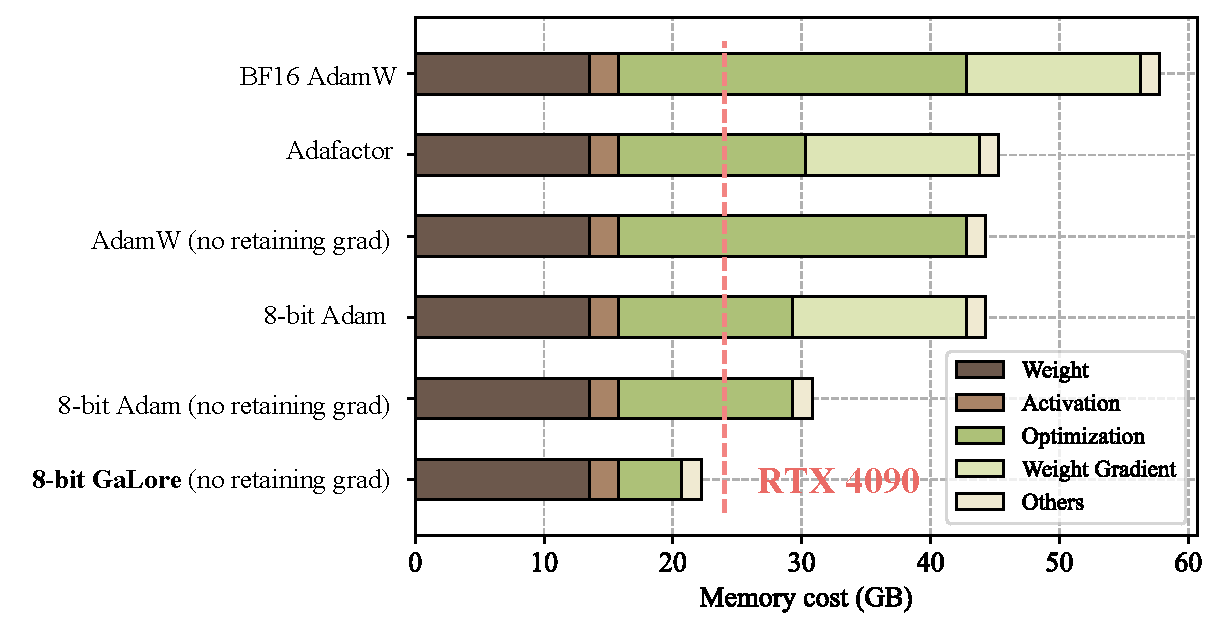
\includegraphics[width=1\columnwidth]{figures/files/memory_breakdown.pdf}
\vskip -0.11in
\caption{\small{Estimated memory consumption of pre-training a LLaMA 7B model with a token batch size of 256 on a single device, without activation checkpointing and memory offloading\protect\footnotemark[2]. Details refer to Section~\ref{sec:memory_measure}.}}
\label{fig:memory_breakdown} 
\vskip -0.15in
\end{figure}
\footnotetext[1]{The calculation is based on LLaMA architecture, BF16 numerical format, and maximum sequence length of 2048.}
\footnotetext[2]{In the figure, ``no retaining grad'' denotes the application of per-layer weight update to reduce memory consumption of storing weight gradient \citep{lvFullParameterFinetuning2023}.}
\SetAlFnt{\fontsize{8pt}{9pt}\selectfont}
\SetAlCapFnt{\fontsize{8pt}{9pt}\selectfont}
\begin{algorithm}[t]
    \SetAlgoLined
        \PyCode{for weight in model.parameters():} \\
        \Indp   %
            \PyCode{grad = weight.grad} \\ 
            \PyComment{original space -> compact space} \\
            \PyCode{lor\_grad = \textbf{project}(grad)} \\
            \PyComment{update by Adam, Adafactor, etc.} \\
            \PyCode{lor\_update = \textbf{update}(lor\_grad)} \\
            \PyComment{compact space -> original space} \\
            \PyCode{update = \textbf{project\_back}(lor\_update)} \\
            \PyCode{weight.data += update} \\
        \Indm %
    \caption{\fontsize{8pt}{9pt}\selectfont{\lowrank{}, PyTorch-like}}
    \label{alg:code_box}
\end{algorithm}


However, the performance of GaLore is still not on par with the Adam or AdamW optimization on the original space. To bridge this gap, we propose \lowrank, which uses the full empirical Fisher Information matrix, thereby incorporating the missing second-order interaction information in the optimization process. This leads to a much more favorable dependence on the starting point, which means that they can make much more progress given a limited iteration budget. Further, when using a decaying learning rate schedule like with AdamW (reference), the asymptotic convergence rate can by faster by a large constant factor.

\subsection{\lowrank and Fisher Efficiency}

Natural gradient methods are optimization algorithms that adjust parameter updates according to the geometry of the parameter space, leading to faster convergence compared to standard gradient descent \citep{amariNaturalGradientWorks1998}. They precondition the gradient using the inverse of the Fisher Information Matrix (FIM), effectively incorporating second-order information about the loss landscape.

The key difference between GaLore and \lowrank is that the gradient update using popular optimizers like Adam, AdamW, etc is applied to the preconditioned gradient:
\[
\tilde{g} = \mathbf{F}^{-1} \mathbf{g}
\]
where \( F(\theta^*) \) is the Fisher Information Matrix, leaving the choice of the projection matrix $\mathbf{P}$ exactly the same.

Fortunately, natural gradient descent is known \citep{martens2020new} for its desirable property of being \textit{Fisher Efficient}, exactly under the condition that the loss function can be represented in terms of KL divergence between the true and approximated distributions i.e. the CLM objective \ref{eq:cross_entropy_loss}. Fisher efficiency means that the natural gradient estimator achieves the lowest possible variance among all unbiased estimators of the gradient.

For \lowrank, the gradient descent update \ref{eq:gradient_descent_update} leads to a sequence of estimates \( \theta_k \) whose variance satisfies \citep{amariNaturalGradientWorks1998}:
\[
\text{Var}[\theta_{k}] = \frac{1}{mk} F^{-1}(\theta_{k}^*) + \mathcal{O}\left(\frac{1}{k^2}\right)
\]
which is asymptotically the smallest possible variance matrix, i.e. the Cramér-Rao lower bound, that any unbiased estimator computed from \(mk\) training samples can have, with \(m\) as the batch size. Here \(\theta_{k}^*\) is the local optima, in the neighborhood defined by the Taylor series expansion around the update. (See more)

Although natural gradient descent is often considered the optimal optimization method in stochastic settings due to its Fisher efficiency, several significant caveats and conditions accompany this result.

First, the proof of Fisher efficiency assumes that the parameter updates converge to the global optimum \( \theta^* \). While this assumption holds in convex optimization problems, it does not generally hold for non-convex objectives commonly encountered in deep neural networks. In practice, convergence may only reach a local optimum, and the Fisher efficiency property may only hold approximately, if at all. Change this paragraph to reflect that at each step we doing a local optimization.

Second, the result relies on the exact computation of the Fisher Information Matrix \( F(\theta) \) using the entire data distribution. In large-scale machine learning tasks, computing \( F(\theta) \) over the entire training set is computationally infeasible. Approximating \( F(\theta) \) using mini-batches or running estimates introduces errors that may invalidate the Fisher efficiency guarantee.

Third, the Fisher efficiency result focuses on the convergence of the parameter estimates \( \theta_k \) in terms of their variance, rather than directly addressing the convergence of the objective function value \( h(\theta_k) \). While reducing variance in parameter estimates is beneficial, practitioners are often more interested in the optimization of the loss function itself. The relationship between parameter variance and loss convergence is not straightforward and may depend on additional assumptions. not important.

Finally, the proof assumes that the model is capable of perfectly capturing the true data distribution—a condition known as \emph{realizability}. This means that at the optimal parameters \( \theta^* \), the model distribution matches the data distribution exactly. In practice, models may be misspecified or lack sufficient capacity to fully represent the true data distribution, violating this assumption and potentially invalidating the Fisher efficiency result. Bigger LLMs are more likely to be realizable.

Despite these caveats, natural gradient descent remains a valuable optimization method, especially when the iteration budget is limited. There are several reasons for this:

First, natural gradient descent can offer \textbf{improved convergence rates in practice}. Even if the asymptotic guarantees are compromised due to the aforementioned conditions, incorporating second-order information through the Fisher Information Matrix—or its approximation—allows the optimizer to account for the curvature of the loss landscape. This enables natural gradient descent to take more informed steps compared to standard gradient descent, potentially escaping flat regions or navigating steep ravines more effectively.

Second, there is \textbf{enhanced performance with limited iterations}. In practical scenarios where computational resources or time limit the number of allowable iterations, the benefits of incorporating second-order information become more pronounced. Natural gradient descent can achieve lower loss values or better parameter estimates within a fixed iteration budget compared to first-order methods, even if the asymptotic variance reduction is not fully realized.

Third, natural gradient descent can lead to a \textbf{reduction of the starting point dependent term} in convergence. While asymptotically the difference in performance between natural gradient descent and simpler methods may diminish, natural gradient descent can significantly reduce the constant factors associated with convergence terms that depend on the initial parameter values. This reduction can result in practical performance gains in finite-iteration regimes.

Finally, the method allows for the \textbf{approximate usage of the Fisher Information Matrix}. Although computing the exact Fisher Information Matrix is infeasible for large models, practical approximations or efficient estimations—such as using a limited history of gradients or employing block-diagonal or low-rank approximations—can capture sufficient curvature information to improve optimization without incurring prohibitive computational costs.

In conclusion, while the theoretical Fisher efficiency of natural gradient descent comes with significant assumptions that may not hold in practical settings, the method still offers substantial advantages when the number of iterations is limited. By leveraging curvature information, natural gradient descent can provide faster convergence and better optimization performance in the early stages of training large-scale models, making it a valuable tool in the machine learning practitioner's arsenal.


\begin{enumerate}
    \item \textbf{Low-Rank Gradient Projection}
    \item \textbf{Gradient History Buffer Maintenance}
    \item \textbf{FIM Approximation Using Gradient History}
    \item \textbf{Natural Gradient Computation via Woodbury Identity}
    \item \textbf{Efficient Solution Using Cholesky Decomposition}
\end{enumerate}

We explain each step in detail below.

\paragraph{Step 1: Low-Rank Gradient Projection}

\begin{algorithm}[t]
  \SetAlgoLined
  \PyCode{def \textbf{project}(full\_rank\_grad, iter):} \\
  \Indp   %
      \PyComment{Check if projection matrices need updating} \\
      \PyCode{\textbf{if} core is None \textbf{or} iter \% update\_proj\_gap == 0:} \\
      \Indp   %
          \PyCode{core, factors = get\_orthogonal\_matrix(full\_rank\_grad, rank)} \\
      \Indm   %
      \PyComment{Transform gradient to low-rank space} \\
      \PyCode{low\_rank\_grad = transform(factors, full\_rank\_grad)} \\
      \PyComment{Apply natural gradient transform} \\
      \PyCode{low\_rank\_grad = \textbf{natural\_gradient\_transform}(low\_rank\_grad)} \\
      \PyCode{\textbf{return} low\_rank\_grad} \\
  \Indm   %
  \caption{\fontsize{8pt}{9pt}\selectfont{Pseudocode for \textbf{project} method}}
  \label{alg:project_method}
\end{algorithm}


Given a full-rank gradient tensor $\mathbf{g} \in \mathbb{R}^{n_1 \times n_2 \times \cdots \times n_d}$, we project it onto a low-rank subspace using Tucker decomposition \citep{tuckerMathematicalNotesThree1966}. The Tucker decomposition approximates $\mathbf{g}$ as:

\[
\mathbf{g} \approx \mathcal{G} = \mathcal{C} \times_1 \mathbf{U}^{(1)} \times_2 \mathbf{U}^{(2)} \times_3 \cdots \times_d \mathbf{U}^{(d)},
\]

where:

\begin{itemize}
    \item $\mathcal{C} \in \mathbb{R}^{r_1 \times r_2 \times \cdots \times r_d}$ is the core tensor capturing the interaction between different modes.
    \item $\mathbf{U}^{(i)} \in \mathbb{R}^{n_i \times r_i}$ are the factor matrices (often orthogonal), representing the principal components along each mode.
    \item $\times_i$ denotes the mode-$i$ tensor-matrix product.
    \item $r_i$ is the rank along mode $i$, with $r_i \ll n_i$.
\end{itemize}

The transformed low-rank gradient is obtained by projecting $\mathbf{g}$ onto the subspace spanned by $\{\mathbf{U}^{(i)}\}$:

\[
\mathbf{g}_{\text{low}} = \text{Transform}(\mathbf{g}) = \mathbf{g} \times_1 (\mathbf{U}^{(1)})^\top \times_2 (\mathbf{U}^{(2)})^\top \times_3 \cdots \times_d (\mathbf{U}^{(d)})^\top.
\]

This results in a compact representation of the gradient in the low-rank subspace.

\paragraph{Step 2: Gradient History Buffer Maintenance}

\begin{algorithm}[t]
  \SetAlgoLined
  \PyCode{def \textbf{natural\_gradient\_transform}(low\_rank\_grad):} \\
  \Indp   %
      \PyComment{Flatten low-rank gradient to vector} \\
      \PyCode{grad\_vector = low\_rank\_grad.reshape(-1)} \\
      \PyComment{Update gradient history buffer} \\
      \PyCode{append grad\_vector to grad\_history} \\
      \PyCode{\textbf{if} len(grad\_history) > history\_size:} \\
      \Indp   %
          \PyCode{remove oldest gradient from grad\_history} \\
      \Indm   %
      \PyComment{Form matrix G from gradient history} \\
      \PyCode{G = stack(grad\_history)} \\
      \PyComment{Compute S = I + $\lambda^{-1}$ G$^\top$G} \\
      \PyCode{S = (1 / lambda\_damping) * (G$^\top$ @ G)} \\
      \PyCode{add 1.0 to diagonal elements of S} \\
      \PyComment{Compute G$^\top$ grad\_vector} \\
      \PyCode{GTg = G$^\top$ @ grad\_vector} \\
      \PyComment{Solve S z = GTg for z using Cholesky decomposition} \\
      \PyCode{L = Cholesky\_decompose(S)} \\
      \PyCode{solve L u = GTg for u} \\
      \PyCode{solve L$^\top$ z = u for z} \\
      \PyComment{Compute natural gradient} \\
      \PyCode{G\_z = G @ z} \\
      \PyCode{ng\_vector = (1 / lambda\_damping) * grad\_vector} \\
      \PyCode{ng\_vector -= (1 / lambda\_damping$^2$) * G\_z} \\
      \PyComment{Reshape back to original low-rank shape} \\
      \PyCode{natural\_grad = ng\_vector.reshape\_as(low\_rank\_grad)} \\
      \PyCode{\textbf{return} natural\_grad} \\
  \Indm   %
  \caption{\fontsize{8pt}{9pt}\selectfont{Pseudocode for \textbf{natural\_gradient\_transform}}}
  \label{alg:natural_gradient_method}
\end{algorithm}


To capture local curvature information, we maintain a buffer of recent transformed gradients. Let $\mathbf{g}_t$ be the transformed low-rank gradient at iteration $t$, flattened into a vector:

\[
\mathbf{g}_t \in \mathbb{R}^{k}, \quad \text{where } k = r_1 r_2 \cdots r_d.
\]

We store the recent $s$ gradients in the matrix $\mathbf{G}$:

\[
\mathbf{G} = [\mathbf{g}_{t - s + 1}, \mathbf{g}_{t - s + 2}, \dots, \mathbf{g}_t] \in \mathbb{R}^{k \times s}.
\]

This gradient history captures the directions of recent updates, which are informative for approximating the FIM.

\paragraph{Step 3: Approximating the Fisher Information Matrix}

We approximate the Fisher Information Matrix within the low-rank subspace using the outer products of the stored gradients:

\[
\mathbf{F} = \lambda \mathbf{I}_k + \mathbf{G} \mathbf{G}^\top,
\]

where:

\begin{itemize}
    \item $\lambda > 0$ is a damping (regularization) term to ensure numerical stability.
    \item $\mathbf{I}_k$ is the $k \times k$ identity matrix.
\end{itemize}

This approximation is motivated by the empirical Fisher Information Matrix, which can be estimated using gradients observed during training \citep{martensNewPerspectiveNatural2014}.

\paragraph{Step 4: Computing the Natural Gradient via Woodbury Identity}

Computing $\mathbf{F}^{-1}$ directly is computationally expensive for large $k$. We employ the \textbf{Woodbury identity} to compute the inverse efficiently:

\[
\mathbf{F}^{-1} \mathbf{g}_t = \frac{1}{\lambda} \left( \mathbf{g}_t - \mathbf{G} \left( \lambda \mathbf{I}_s + \mathbf{G}^\top \mathbf{G} \right)^{-1} \mathbf{G}^\top \mathbf{g}_t \right).
\]

Defining:

\begin{itemize}
    \item $\mathbf{S} = \lambda \mathbf{I}_s + \mathbf{G}^\top \mathbf{G} \in \mathbb{R}^{s \times s}$.
    \item $\mathbf{y} = \mathbf{G}^\top \mathbf{g}_t \in \mathbb{R}^s$.
\end{itemize}

We compute the natural gradient as:

\begin{enumerate}
    \item Compute $\mathbf{S} = \lambda \mathbf{I}_s + \mathbf{G}^\top \mathbf{G}$.
    \item Solve $\mathbf{S} \mathbf{z} = \mathbf{y}$ for $\mathbf{z}$.
    \item Compute $\tilde{\mathbf{g}}_t = \dfrac{1}{\lambda} \left( \mathbf{g}_t - \mathbf{G} \mathbf{z} \right)$.
\end{enumerate}

This avoids inverting the large matrix $\mathbf{F}$ directly, reducing computational complexity.

\paragraph{Step 5: Efficient Solution Using Cholesky Decomposition}

To solve the linear system $\mathbf{S} \mathbf{z} = \mathbf{y}$ efficiently, we use \textbf{Cholesky decomposition}:

\begin{enumerate}
    \item Compute the Cholesky factorization of $\mathbf{S}$:

    \[
    \mathbf{S} = \mathbf{L} \mathbf{L}^\top,
    \]

    where $\mathbf{L}$ is a lower triangular matrix.

    \item Solve for $\mathbf{u}$ via forward substitution:

    \[
    \mathbf{L} \mathbf{u} = \mathbf{y}.
    \]

    \item Solve for $\mathbf{z}$ via backward substitution:

    \[
    \mathbf{L}^\top \mathbf{z} = \mathbf{u}.
    \]
\end{enumerate}

Cholesky decomposition is efficient for symmetric positive-definite matrices and numerically stable.

\paragraph{Step 6: Updating the Model Parameters}

\begin{algorithm}[t]
  \SetAlgoLined
  \PyCode{def \textbf{project\_back}(low\_rank\_update):} \\
  \Indp   %
      \PyComment{Reconstruct full-rank update from low-rank update} \\
      \PyCode{full\_rank\_update = inverse\_transform(factors, low\_rank\_update)} \\
      \PyComment{Apply scaling if necessary} \\
      \PyCode{\textbf{return} full\_rank\_update * scale} \\
  \Indm   %
  \caption{\fontsize{8pt}{9pt}\selectfont{Pseudocode for \textbf{project\_back} methods}}
  \label{alg:project_back_method}
\end{algorithm}


Finally, we use the natural gradient $\tilde{\mathbf{g}}_t$ to update the model parameters in the low-rank subspace. The full-rank update can be reconstructed using the inverse transformation if necessary.

\subsection{Algorithm Summary}

At each iteration $t$, the algorithm proceeds as follows:

\begin{enumerate}
    \item \textbf{Project the Full-Rank Gradient}:

    \begin{itemize}
        \item Compute the low-rank transformed gradient $\mathbf{g}_t$ using the current factor matrices $\{\mathbf{U}^{(i)}\}$.
    \end{itemize}

    \item \textbf{Update Gradient History}:

    \begin{itemize}
        \item If the history buffer is full, remove the oldest gradient.
        \item Append $\mathbf{g}_t$ to the history buffer $\mathbf{G}$.
    \end{itemize}

    \item \textbf{Compute Intermediate Quantities}:

    \begin{itemize}
        \item $\mathbf{S} = \lambda \mathbf{I}_s + \mathbf{G}^\top \mathbf{G}$.
        \item $\mathbf{y} = \mathbf{G}^\top \mathbf{g}_t$.
    \end{itemize}

    \item \textbf{Solve for $\mathbf{z}$}:

    \begin{itemize}
        \item Use Cholesky decomposition to solve $\mathbf{S} \mathbf{z} = \mathbf{y}$.
    \end{itemize}

    \item \textbf{Compute the Natural Gradient}:

    \begin{itemize}
        \item $\tilde{\mathbf{g}}_t = \dfrac{1}{\lambda} \left( \mathbf{g}_t - \mathbf{G} \mathbf{z} \right)$.
    \end{itemize}

    \item \textbf{Update the Parameters}:

    \begin{itemize}
        \item Use $\tilde{\mathbf{g}}_t$ to update the model parameters in the low-rank subspace.
        \item Optionally, reconstruct the full gradient if necessary for parameter updates.
    \end{itemize}
\end{enumerate}

\subsection{Implementation Details}

\subsubsection{Avoiding Large Matrix Inversions}

By utilizing the Woodbury identity, we reduce the inversion of a large $k \times k$ matrix to the inversion of a much smaller $s \times s$ matrix, where $s$ (the history size) is typically small (e.g., $s = 10$). This makes the computation tractable even for large models.

\subsubsection{Computational Efficiency}

\begin{itemize}
    \item \textbf{Matrix-Vector Products}: We prioritize matrix-vector operations over matrix-matrix multiplications to enhance computational efficiency on GPUs.
    \item \textbf{GPU Acceleration}: All computations are performed on GPUs to leverage parallel processing capabilities and minimize data transfer overhead.
    \item \textbf{Optimized Linear Algebra Libraries}: We employ optimized GPU routines (e.g., cuBLAS, cuSOLVER) for linear algebra operations like matrix multiplication and Cholesky decomposition.
\end{itemize}

\subsubsection{Memory Efficiency}

The additional memory overhead is minimal due to:

\begin{itemize}
    \item \textbf{Small History Size}: Keeping $s$ small limits the size of $\mathbf{G}$ and related matrices.
    \item \textbf{Low-Rank Representation}: Operating in the low-rank subspace significantly reduces the dimensionality of the gradients and the FIM approximation.
\end{itemize}

\subsubsection{Numerical Stability}

The damping term $\lambda$ ensures that $\mathbf{S}$ remains positive definite, which is crucial for the stability of Cholesky decomposition. In practice, $\lambda$ can be treated as a hyperparameter, often set to a small positive value.

\subsubsection{Hyperparameter Selection}

Key hyperparameters include:

\begin{itemize}
    \item \textbf{Rank Parameters} $r_i$: Determines the dimensionality reduction in each mode; chosen based on a trade-off between computational cost and approximation accuracy.
    \item \textbf{History Size} $s$: Controls the amount of curvature information captured; typically small to balance memory usage and performance.
    \item \textbf{Damping Term} $\lambda$: Affects numerical stability and convergence; may require tuning for different models or datasets.
\end{itemize}

\subsection{Theoretical Justification}

Our method leverages the observation that gradients in deep learning often reside in a low-dimensional subspace due to the inherent redundancy in neural network parameterizations and correlations in the data \citep{gurariReducingTrainingTime2021}. By maintaining a history of low-rank gradients, we capture the principal components that approximate the local curvature of the loss surface.

Incorporating second-order information via the inverse FIM improves convergence rates, especially in regimes with limited iteration budgets. The use of the Woodbury identity allows us to efficiently compute the natural gradient in this low-rank subspace, effectively approximating the benefits of full natural gradient methods without their prohibitive computational costs.

\subsection{Empirical Evaluation}

We validate the effectiveness of Natural GaLore through empirical pre-training on LLaMA models with 60M, 300M, and 1.1B parameters using the C4 dataset \citep{raffelExploringLimitsTransfer2020}. Our experiments demonstrate that:

\begin{itemize}
    \item \textbf{Improved Convergence}: Natural GaLore achieves significantly lower perplexity compared to GaLore, indicating faster convergence.
    \item \textbf{Memory Efficiency}: The method incurs no additional memory overhead compared to GaLore, maintaining the advantages of low memory usage.
    \item \textbf{Performance Parity with Standard Optimizers}: The gap between our method and standard optimizers like Adam or AdamW is narrowed, demonstrating competitive performance.
\end{itemize}

\subsection{Conclusion}

We have introduced Natural GaLore, an efficient online natural gradient algorithm that operates in a low-rank subspace of the gradient space. By approximating the inverse Empirical Fisher Information Matrix using the Woodbury identity and maintaining a history of low-rank gradients, we incorporate second-order information into the optimization process without significant computational or memory overhead. Our method addresses the limitations of GaLore by improving convergence rates and achieving performance closer to that of standard optimizers, making it suitable for training large-scale language models under memory constraints.


\section{\lowrank: Gradient Low-Rank Projection}
\subsection{Background}


\textbf{Regular full-rank training.} At time step $t$, $G_t = -\nabla_W \phi_t(W_t) \in \mathbb{R}^{m \times n}$ is the backpropagated (negative) gradient matrix. Then the regular pre-training weight update can be written down as follows ($\eta$ is the learning rate):
\begin{equation}
    W_T = W_0 + \eta \sum_{t=0}^{T-1} \tilde G_{t} = W_0 + \eta\sum_{t=0}^{T-1} \rho_t(G_t)
\end{equation}
where $\tilde G_t$ is the final processed gradient to be added to the weight matrix and $\rho_t$ is an entry-wise stateful gradient regularizer (e.g., Adam). The state of $\rho_t$ can be memory-intensive. For example, for Adam, we need $M,V \in \mathbb{R}^{m\times n}$ to regularize the gradient $G_t$ into $\tilde G_{t}$:
\begin{eqnarray}
    M_t &=& \beta_1 M_{t-1} + (1-\beta_1) G_t \\
    V_t &=& \beta_2 V_{t-1} + (1-\beta_2) G^2_t  \\
    \tilde G_t &=& M_t / \sqrt{V_t + \epsilon}
\end{eqnarray}
Here $G_t^2$ and $M_t / \sqrt{V_t + \epsilon}$ means element-wise multiplication and division. $\eta$ is the learning rate. Together with $W\in \mathbb{R}^{m\times n}$, this takes $3mn$ memory.

From the theoretical analysis above, we can see that for batch size $N$, the gradient $G$ has certain structures: $G = \frac{1}{N}\sum_{i=1}^N (A_i - B_i W C_i)$ for input-dependent matrix $A_i$, Positive Semi-definite (PSD) matrices $B_i$ and $C_i$. In the following, we prove that such a gradient will become low-rank during training in certain conditions:

\def\sr{\mathrm{sr}}

\begin{restatable}[Gradient becomes low-rank during training]{lemma}{gradientlowrank}
\label{lemma:gradientlowrank}
    Suppose the gradient follows the parametric form:
    \begin{eqnarray}
          G_t=\frac{1}{N}\sum_{i=1}^N (A_i-B_i W_t C_i)\label{eq:constantgradientcoeff}
    \end{eqnarray}
    with constant $A_i$, PSD matrices $B_i$ and $C_i$ after $t \ge t_0$. We study vanilla SGD weight update: $W_t=W_{t-1}+\eta G_{t-1}$. Let $S := \frac{1}{N}\sum_{i=1}^N C_i \otimes B_i$ and $\lambda_1 < \lambda_2$ its two smallest distinct eigenvalues. Then the stable rank $\sr(G_t)$ satisfies:
    \begin{equation}
        \sr(G_t) \le \sr(\gzeroproj)\!+\!\left(\frac{1\!-\!\eta \lambda_2}{1\!-\!\eta \lambda_1}\right)^{2(t-t_0)} \frac{\|G_0\!-\!\gzeroproj\|_F^2}{\|\gzeroproj\|_2^2} \label{eq:stable-rank-decay}
    \end{equation}
    where $\gzeroproj$ is the projection of $G_{t_0}$ onto the minimal eigenspace $\cV_1$ of $S$ corresponding to $\lambda_1$.
\end{restatable}

In practice, the constant assumption can approximately hold for some time, in which the second term in Eq.~\ref{eq:stable-rank-decay} goes to zero exponentially and the stable rank of $G_t$ goes down, yielding low-rank gradient $G_t$. The final stable rank is determined by $\sr(\gzeroproj)$, which is estimated to be low-rank by the following:
\begin{restatable}[Low-rank $G_t$]{corollary}{lowrankmid}
\label{co:low-rank-mid}
If the gradient takes the parametric form $G_t = \frac{1}{N}\sum_{i=1}^N (\va_i - B_i W_t \vf_i)\vf_i^\top$ with all $B_i$ full-rank, and $N' := \rank(\{\vf_i\}) < n$, then $\sr(\gzeroproj) \le n - N'$ and thus $\sr(G_t) \le n/2$ for large $t$.
\end{restatable}

\textbf{Transformers.} For Transformers, we can also separately prove that the weight gradient of the lower layer (i.e., \emph{project-up}) weight of feed forward network (FFN) becomes low rank over time, using the JoMA framework~\cite{tian2023joma}. Please check Appendix (Sec.~\ref{sec:transformer-low-rank}) for details.

\section{\lowrank{} for Memory-Efficient Training}
For a complex optimization problem such as LLM pre-training, it may be difficult to capture the entire gradient trajectory with a single low-rank subspace. One reason is that the principal subspaces of $B_t$ and $C_t$ (and thus $G_t$) may change over time. In fact, if we keep the same projection $P$ and $Q$, then the learned weights will only grow along these subspaces, which is not longer full-parameter training. Fortunately, for this, \lowrank{} can switch subspaces during training and learn full-rank weights without increasing the memory footprint.

\textbf{Reducing memory footprint of gradient statistics.} \lowrank{} significantly reduces the memory cost of optimizer that heavily rely on component-wise gradient statistics, such as Adam \citep{kingmaAdamMethodStochastic2014}.

\subsection{Combining with Existing Techniques}

\lowrank{} is compatible with existing memory-efficient optimization techniques. For example, \lowrank{} can be combined with gradient checkpointing \citep{chenTrainingDeepNets2016} to further reduce memory usage.


\subsection{Hyperparameters of \lowrank{}}
\label{sec:lowrank-hyperparams}
In addition to Adam's original hyperparameters, \lowrank{} only introduces very few additional hyperparameters: the rank $r$ which is also present in LoRA, the subspace change frequency $T$ (see Sec.~\ref{sec:composition-subspace}), and the scale factor $\alpha$.

Scale factor $\alpha$ controls the strength of the low-rank update, which is similar to the scale factor $\alpha/r$ appended to the low-rank adaptor in \citet{huLoRALowRankAdaptation2021}.
We note that the $\alpha$ does not depend on the rank $r$ in our case.
This is because, when $r$ is small during pre-training, $\alpha/r$ significantly affects the convergence rate, unlike fine-tuning.

\begin{table}[t]
    \caption{\small{Comparison between \lowrank{} and LoRA. Assume $W \in \mathbb{R}^{m \times n}$ ($m \leq n$), rank $r$.}}
    
    \label{tab:lora_compare}
    \begin{center}
    \begin{small}
    \begin{tabular}{lcc}
    \toprule
               & \lowrank{} & LoRA \\
    \midrule
    Weights          & $mn$   & $mn+mr+nr$ \\
    Optim States           & $mr + 2nr$   & $2mr + 2nr$  \\
    \midrule
    Multi-Subspace   & \cmark   & \xmark \\
    Pre-Training   & \cmark   & \xmark \\
    Fine-Tuning   & \cmark   & \cmark \\
    \bottomrule
    \end{tabular}
    \end{small}
    \end{center}
\vspace{-6mm}
\end{table}


\section{Experiments}

We evaluate \textit{\lowrank} on pre-training and fine-tuning tasks for LLMs. All experiments are conducted on a single node with 8 NVIDIA A100 GPUs to leverage high-performance computing capabilities, yet stay within reasonable limits.

\subsection{Pre-training on the C4 Dataset}

To assess the effectiveness of \textit{\lowrank}, we apply it to pre-train LLaMA-based language models of sizes ranging from 60 million to 1.1 billion parameters, on the C4 dataset. The C4 dataset is a colossal, cleaned version of the Common Crawl Corpus, primarily intended for pre-training language models and word representations \citep{raffelExploringLimitsTransfer2020}. It provides a diverse and extensive corpus, making it suitable for evaluating pre-training methods in realistic scenarios.

We adopt the experimental setup from \citet{lialinReLoRAHighRankTraining2023}, utilizing a LLaMA-based\footnote[2]{LLaMA materials in our paper are subject to the LLaMA community license.} architecture with RMSNorm and SwiGLU activations \citep{shazeerGLUVariantsImprove2020,touvronLlamaOpenFoundation2023}. We maintain the same set of hyperparameters for each model size across all methods, except for the learning rate, which is tuned individually to ensure optimal performance. All experiments use the BF16 format to reduce memory usage without compromising computational efficiency, the same computational budget and the best validation perplexity is reported.

\begin{figure}[ht]
    \centering
    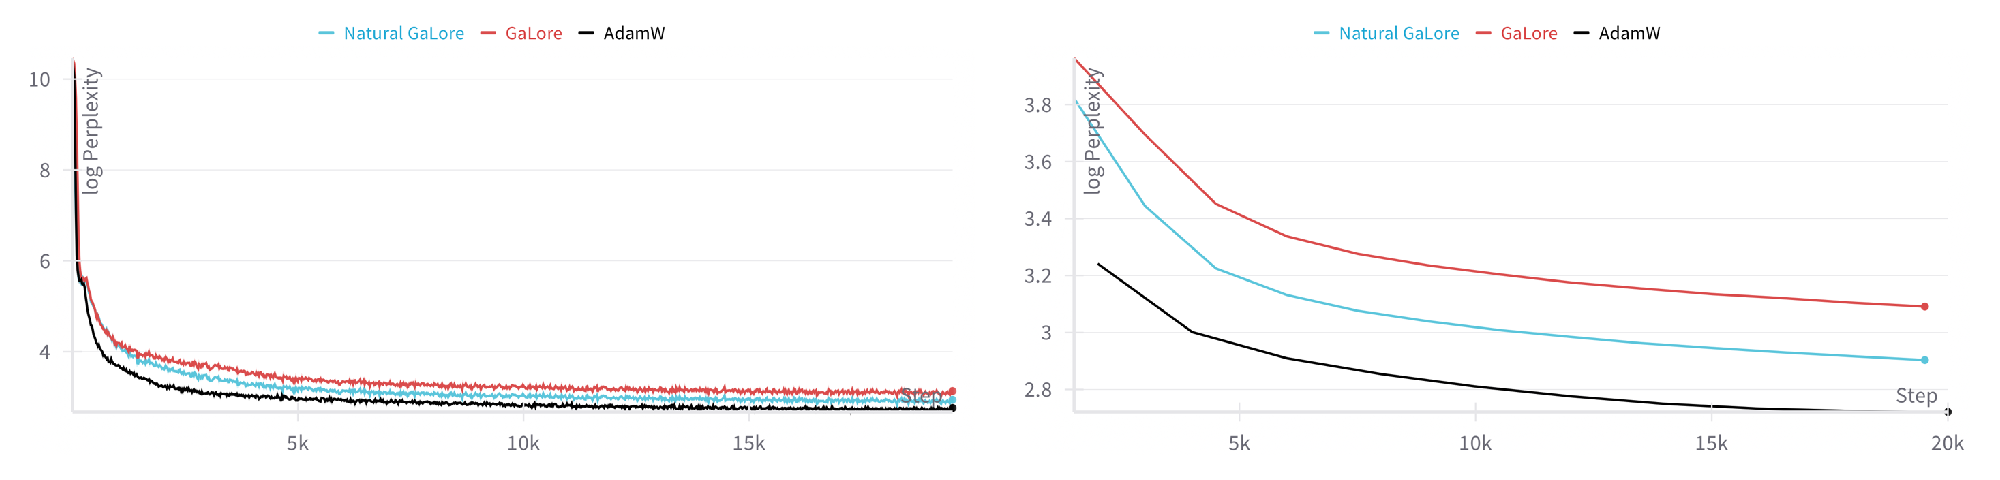
\includegraphics[width=\linewidth]{figures/train_and_validate_llama1_1B.pdf}
    \vspace{-4.5mm}
    \caption{\small{Training and Validation log Perplexity for Llama 1.1B.
    }}
    \vspace{-4mm}
    \label{fig:train_loss}
\end{figure}

\begin{table*}[ht]
    \centering
    \caption{\small{Comparison of \lowrank with other low-rank algorithms on pre-training various sizes of LLaMA models on the C4 dataset. Validation log perplexity is reported, along with a memory estimate (in gigabytes) of the total parameters and optimizer states based on BF16 format.}}
    \label{tab:lora_compare_llama}
    \begin{tabular}{lcccc}
    \toprule
                     & \textbf{60M} & \textbf{130M} & \textbf{350M} & \textbf{1.1B} \\
    \midrule
    Full-Rank        & 3.52 (0.36G) & 3.22 (0.76G) & 2.93 (2.06G) & 2.72 (7.80G) \\
    \midrule
    \lowrank & \textbf{3.53} (0.24G) & \textbf{3.22} (0.52G) & \textbf{2.93} (1.22G) & \textbf{2.80} (4.38G) \\
    GaLore           & 3.56 (0.24G) & 3.24 (0.52G) & 2.95 (1.22G) & 2.90 (4.38G) \\
    Low-Rank         & 4.35 (0.26G) & 3.82 (0.54G) & 3.62 (1.08G) & 4.96 (3.57G) \\
    LoRA             & 3.55 (0.36G) & 3.52 (0.80G) & 3.24 (1.76G) & 2.96 (6.17G) \\
    ReLoRA           & 3.61 (0.36G) & 3.38 (0.80G) & 3.37 (1.76G) & 2.91 (6.17G) \\
    \bottomrule
    Rank $r / d_{\text{model}}$ & 128 / 256 & 256 / 768 & 256 / 1024 & 512 / 2048 \\
    Training Tokens  & 1.1B & 2.2B & 6.4B & 13.1B \\
    \bottomrule
    \end{tabular}
\end{table*}

Table~\ref{tab:lora_compare_llama} presents the validation perplexity and memory consumption for models trained with different methods and Figure~\ref{fig:train_loss} shows the training run for the Llama 1.1B model. Our proposed \textit{\lowrank} consistently outperforms GaLore \citep{zhao2024galore} across all model sizes, achieving validation perplexities closer to the full-rank baseline while maintaining significant memory savings. Furthermore, \textit{\lowrank} exhibits lower perplexities and greater memory consumption compared to other low-rank adaptation methods like LoRA and ReLoRA, due to their less efficient use of low-rank structures and the need for additional optimizer states.

\vspace{-2mm}

\subsection{Fine-Tuning RoBERTa-Base on the GLUE Benchmark}

To further evaluate the effectiveness of \textit{\lowrank}, we conduct experiments on the General Language Understanding Evaluation (GLUE) benchmark using the pre-trained RoBERTa-Base model. The GLUE benchmark is a collection of nine natural language understanding tasks, including single-sentence tasks like CoLA \citep{warstadt2019neural}, similarity and paraphrase tasks like MRPC \citep{dolan2005automatically} and STS-B \citep{cer2017semeval}, and inference tasks like RTE \citep{dagan2005pascal}, MNLI \citep{williams2018broad}, and QNLI \citep{rajpurkar2016squad}. This benchmark is widely used to assess the performance of language models on diverse linguistic phenomena.

In our experiments, we fine-tune the RoBERTa-Base model using \textit{\lowrank} and compare its performance with full fine-tuning and LoRA \citep{huLoRALowRankAdaptation2021}. We focus on memory-efficient fine-tuning methods to reduce the computational footprint while maintaining high performance. For each method, we report the average score across all GLUE tasks and individual task scores.

We use the same training hyperparameters across all methods for a fair comparison. The batch size is 32, and we fine-tuned each model for three epochs. The learning rate is selected from \{1e-5, 2e-5, 3e-5\} based on the best validation performance for each task. For \textit{\lowrank} and LoRA, we experiment with rank values of 4 and 8 to study the trade-off between performance and memory efficiency.

Table~\ref{tab:fine_tuning} presents the results of our experiments. \textit{\lowrank} consistently achieves comparable or better performance than LoRA across most tasks while using less memory. Precisely, with a rank of 4, \textit{\lowrank} attains an average score of \textbf{86.05}, closely matching the complete fine-tuning baseline of 86.28 and outperforming LoRA's average score of 85.61. This demonstrates that \textit{\lowrank} can effectively fine-tune large models with reduced memory consumption without sacrificing performance.

\begin{table}[t]
    \caption{\small Evaluating \lowrank{} for memory-efficient fine-tuning on GLUE benchmark using pre-trained RoBERTa-Base. We report the average score of all tasks.}
    \label{tab:fine_tuning}
    \centering
    \resizebox{\linewidth}{!}{%
    \begin{tabular}{l|c|cccccccc|c}
    \toprule
               & \textbf{Memory} & \textbf{CoLA} & \textbf{STS-B} & \textbf{MRPC} & \textbf{RTE} & \textbf{SST2} & \textbf{MNLI} & \textbf{QNLI} & \textbf{QQP} & \textbf{Avg} \\
    \midrule
    Full Fine-Tuning & 747M & 62.24 & 90.92 & 91.30 & 79.42 & 94.57 & 87.18 & 92.33 & 92.28 & 86.28 \\
    \midrule
    \textbf{\lowrank{} (rank=4)} & 253M & 60.35 & \textbf{90.73} & \textbf{92.25} & \textbf{79.42} & \textbf{94.04} & \textbf{87.00} & \textbf{92.24} & 91.06 & \textbf{85.89} \\
    LoRA (rank=4) & 257M & \textbf{61.38} & 90.57 & 91.07 & 78.70  & 92.89 & 86.82 & 92.18 & \textbf{91.29} & 85.61 \\
    \midrule
    \textbf{\lowrank{} (rank=8)} & 257M & 60.06 & \textbf{90.82} & \textbf{92.01} & \textbf{79.78} & \textbf{94.38} & \textbf{87.17} & 92.20 & 91.11 & \textbf{85.94} \\
    LoRA (rank=8) & 264M & \textbf{61.83} & 90.80 & 91.90 & 79.06  & 93.46 & 86.94 & \textbf{92.25} & \textbf{91.22} & 85.93 \\
    \bottomrule
    \end{tabular}
    }
    \vskip -0.1in
\end{table}





\vspace{-2mm}

\subsection{Fine-Tuning TinyLlama 1.1B for Function Calling in Advanced Agentic Systems}

Advanced Agentic Systems (AAS) require language models that can understand and generate code snippets to integrate various tools and APIs, fulfilling user queries through function-calling. We utilize the TinyAgent framework, which provides an end-to-end pipeline for training and deploying task-specific LLM agents capable of efficient and accurate function-calling \citep{erdogan2024tinyagent} to drive agentic systems at the edge.

Given a natural language query, the LLM agent must generate a sequence of pre-defined function-calls that accomplish the desired tasks. The challenge lies in determining the appropriate arguments, to call the correct functions, in the right order while respecting interdependencies among the functions.

LLMCompiler \citet{kim2023llmcompiler}, is a framework that enables language models to perform function-calling by first generating a function-calling plan, which includes the required functions and arguments. The LLMCompiler then compiles this plan into an executable sequence of function-calls. The critical aspect is training the model to produce a function-calling plan with the correct syntax and dependencies.

The off-the-shelf pre-trained TinyLlama 1.1B (instruct-32k) model performs poorly on this task. The model generates incorrect sets of functions, hallucinated function names, fails to respect dependencies, and passes arguments incorrectly. This underperformance is expected, as the model was initially trained on datasets like SlimPajama and StarCoder, which are not specific to function-calling tasks. To address this, we follow the TinyAgent framework \citep{erdogan2024tinyagent} and fine-tune the TinyLlama 1.1B model on a high-quality, curated dataset designed for function-calling.

\paragraph{TinyAgent Dataset}

The TinyAgent dataset \citep{erdogan2024tinyagent} is a meticulously curated collection aimed at building a local agentic system for function-calling on Apple MacBooks for day-to-day tasks. It contains 40K examples of natural language queries and corresponding function-calling plans. The dataset is divided into 38K training examples, 1K validation examples, and 1K test examples. It encompasses 16 tasks, including Email, Contacts, SMS, Calendar, Notes, Reminders, File Management and Zoom Meetings. Each task has predefined scripts that the model needs to generate. The dataset is intentionally challenging, requiring the model to understand dependencies between function-calls and the arguments to be passed.

\paragraph{Fine-Tuning Procedure}

We fine-tune the TinyLlama 1.1B model on the TinyAgent dataset for three epochs using a batch size of 32. The learning rate is set to \(7 \times 10^{-5}\). After each epoch, the model is evaluated on the validation set, and the best-performing model is selected based on validation performance to be evaluated on the test set.

During fine-tuning, the prompt includes descriptions of the ground truth functions and irrelevant functions serving as negative samples. This strategy encourages the model to learn to select the correct functions rather than merely memorizing the ground truth. Additionally, several in-context examples demonstrate how queries are translated into function-calling plans. These examples are selected using a Retrieval-Augmented Generation (RAG) process based on the user's query from the training data and a DeBERTa-v3-small model \citep{he2021debertav3} fine-tuned for multi-label classification for retrieval among the 16 tools.

The training objective is then to maximize the accuracy of the generated function-calling plans. Success is defined by the model generating the correct plan with the proper set of function-calls, correct arguments, and the appropriate order of function-calls. Verifying the selection of the correct set of functions involves straightforward set comparison. However, ensuring the correctness of arguments and the order of function-calls is more complex and requires constructing the associated Directed Acyclic Graph to check for equality.

\paragraph{Results and Discussion}

\begin{table*}[ht]
\vspace{-3mm}
\caption{
Latency, size, and success rate of TinyAgent models before and after quantization. Latency is the end-to-end latency of the function calling planner, including the prompt processing time and generation.}
\vspace{-1mm}
\begin{center}
\small{
\setlength{\tabcolsep}{6pt}{
\begin{tabular}{c|c|c|c|c}
\toprule
Model &	Weight Precision &	Latency (seconds)	& Model Size (GB)	& Success Rate (\%) \\
\midrule
GPT-3.5 & Unknown & 3.2 & Unknown & 65.04 \\
GPT-4-Turbo & Unknown & 3.9 & Unknown & 79.08 \\
\midrule
\multirow{2}{*}{TinyAgent-1.1B} & 16-bit (\textit{\lowrank}) & 3.9 & 2.2 & \textbf{83.09} \\
& 16-bit (LoRA) & 3.9 & 2.2 & 80.06 \\
\midrule
\multirow{1}{*}{TinyAgent-7B} & 16-bit \citep{erdogan2024tinyagent} & 19.5 & 14.5 & 84.95 \\
\bottomrule
\end{tabular}
}
}
\end{center}
\label{table:t2}
\end{table*}




After fine-tuning, the TinyLlama 1.1B model's success rate on the test set improved significantly. Table~\ref{table:t2} presents the latency, model size, and success rate of various models on the TinyAgent dataset. As shown, \textit{\lowrank} improves the success rate of the 1.1B model from 80.06\% (16-bit LoRA) to \textbf{83.09\%}, also surpassing GPT-4-Turbo by 4\% and approaching the performance of the larger TinyAgent-7B model, which achieves 84.95\%.

These results demonstrate that \textit{\lowrank} not only enhances the performance of smaller models like the 1.1B parameter TinyLlama but also makes them competitive with significantly larger models. By efficiently incorporating second-order information through low-rank natural gradient updates, \textit{\lowrank} enables smaller models to achieve higher accuracy without additional memory overhead.

\section{Conclusion}

We have introduced \textit{\lowrank}, a memory-efficient pre-training and fine-tuning strategy for large language models. \textit{\lowrank} significantly reduces memory usage—by up to 65.5\% in optimizer states—while maintaining or even improving performance in large-scale LLM pre-training and fine-tuning tasks. By incorporating second-order information through an efficient approximation of the inverse Empirical Fisher Information Matrix, \textit{\lowrank} enhances convergence rates, especially in regimes with a limited iteration budget.

Importantly, \textit{\lowrank} can serve as a \emph{drop-in replacement} for standard optimizers like AdamW and integrates seamlessly into existing training pipelines. Our experimental results highlight the effectiveness of \textit{\lowrank} across various tasks, including pre-training LLaMA models and fine-tuning on the GLUE benchmark, as well as the TinyAgent function calling tasks. This makes it a compelling choice for large-scale pre-training scenarios where both memory efficiency and model performance are critical.

In the future we want to explore (1) further enhancing memory efficiency by employing low-memory and structured projection matrices, and (2) more extensive empirical evaluation on fine-tuning AAS on a wide variety of tasks. We also hope that our work will inspire future research on memory-efficient training methods from the perspective of optimizer state approximation. We believe that \textit{\lowrank} will be a valuable tool for the community, enabling the training of large-scale models on consumer-grade hardware with limited resources.

\section*{Impact Statement}

This work aims to improve the memory efficiency of training LLMs, thereby reducing the environmental impact of LLM pre-training and fine-tuning. By enabling the training of larger models on hardware with lower memory requirements, our approach helps to minimize energy consumption and carbon footprint associated with training LLMs. Furthermore, by making advanced model training more accessible, we contribute to democratizing AI research and development, allowing a broader community to engage with large-scale models without the need for expensive computational resources.
%\section*{Acknowledgments}

We thank Meta AI for computational
support. 
We appreciate the helpful feedback and discussion from Florian Sch{\"a}fer, Jeremy Bernstein, and Vladislav Lialin.
B. Chen greatly appreciates the support by Moffett AI.
Z. Wang is in part supported by NSF Awards 2145346 (CAREER), 02133861 (DMS), 2113904 (CCSS), and the NSF AI Institute for Foundations of Machine Learning (IFML).
A. Anandkumar is supported by the Bren Foundation and the Schmidt Sciences through AI 2050 senior fellow program.

\bibliography{iclr_template/iclr2025_conference}
\bibliographystyle{iclr_template/iclr2025_conference}

\end{document}
